\subsection{Model}
The \emph{model} represents the business logic to solve the problems listed as the requirements of the systems. Once the use cases outlined in \autoref{chap:requirements} are analyzed, the functions of each system components can be determined and then a sequence of operations can be created for each specific use case.
To gain a better overview and understanding of the entities inside the system, a diagram is created.
\begin{figure}[H]
    \centering
    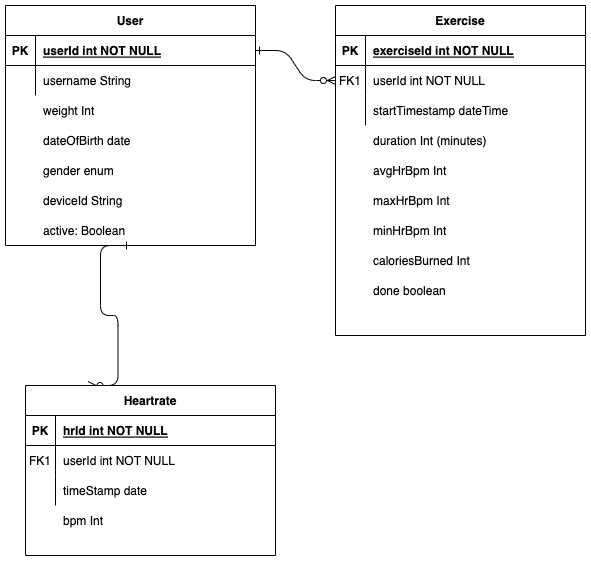
\includegraphics[width=0.8\textwidth]{diagrams/ham-entity.drawio.png}
    \caption{Entity class diagram}
    \label{fig:entity_diagram}
\end{figure}
This diagram illustrates the main entities and its relationship with each other inside the system. As described by the diagram, the main entities in the system consist of \emph{user}, \emph{exercise}, \emph{heartrate}. 
Each \emph{user} within the system has one to many relationship with both \emph{heartrate} and \emph{exercise} entities. These relationships represent the connection between a \emph{user} and their corresponding \emph{heartrate} and \emph{exercise} records. 
Once the entities have been defined, the system's functionalities can now be discussed based on the identified use cases.

\subsubsection{Heart Rate Monitor}
A system sequence can now be defined as a result of analyzing the following use case:
\begin{quotation}
    \enquote{As a health-oriented user, I want the application to show my live heart rate so that I can monitor my cardiovascular activity.} 
\end{quotation}

\begin{figure}[H]
    \centering
    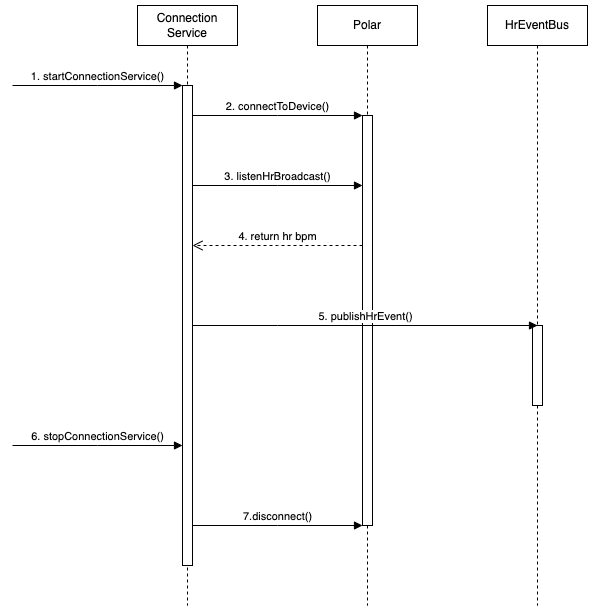
\includegraphics[width=1\textwidth]{diagrams/connection-service-onStart.drawio.png}
    \caption{Connection service sequence diagram}
    \label{fig:connection_diagram}
\end{figure}

The following sequence will be executed as a way to maintain connection to the BLE heart rate sensor and retrieve the heart rate data.
\begin{enumerate}
    \item A request to start the \emph{connection service} is received.
    \item The service initiates a bluetooth low energy connection to the heart rate sensor device.
    \item After the connection has been established, the \emph{connection service} listens to the heart rate data broadcasted by the heart rate sensor device
    \item The heart rate sensor broadcasts heart rate data
    \item The service publishes an event containing the received heart rate data
    \item A request to stop the \emph{connection service} is received.
    \item The service stops the connection with the heart rate sensor device
\end{enumerate}

\subsubsection{Activity Monitor}
Based on the analysis of the following use case, a system sequence that outlines the sequence of actions and interactions within the system can now be established.
\begin{quotation}
    \enquote{As an physically active individuals, I want the application to track and display my current activity so that I can keep track of my progress and make adjustments to my physical activities.} 
\end{quotation}




